\chapter[RASA]{RASA Open Source}
Rasa es un framework que permite la construcción de forma sencilla de chatbots personalizados, está
compuesta de dos librerias de código abierto, Rasa NLU y Rasa Core, denominadas en conjunto Rasa
Stack.
\indent
\section{Conceptos Básicos}
\begin{itemize}
	\item \textbf{intents (intenciones): }son las categorías, denominadas utterances creadas para
	      lo que el usuario está tratando de transmitir o lograr en una conversación, por ejemplo 'saludos'
	      donde se especifican las distintas formas de saludar. Las intenciones pueden ser divididas en
	      pequeñas subintenciones denominadas 'Retrieval Intent'.
	\item \textbf{entities (entidades): } las entidades son informaciones o palabras clave que
	      pueden ser extraídas de un mensaje para personalizar la conversación.
	\item \textbf{slots:} es un registro de datos que Rasa utiliza para guardar la información
	      proveída por el usuario en el curso de la conversación, un claro ejemplo del uso de este elemento
	      es almacenar el nombre del usuario para personalizar los mensajes.
	\item \textbf{responses (respuestas):} mensajes que los chatbots envían a los usuarios, estos
	      pueden ser dinámicos y con cualquier tipo de contenido como texto, imágenes, links, etc.
	\item \textbf{forms (formularios):} Un tipo de acción personalizada que pide al usuario varios
	      datos.
	\item \textbf{actions (acciones):} es un paso que toma el bot en la conversación por ejemplo,
	      llamar a una API o enviar una respuesta al usuario.\cite{Glossary}
\end{itemize}

\section{Cómo se lleva a cabo las conversaciones?}
Para llevar a cabo las conversaciones se utilizan las dos librerías del Rasa Stack.
\begin{itemize}
	\item \textbf{Rasa NLU: } En ella  se escriben los archivos de configuración, se elige el
	      pipeline y el modelo de entrenamiento para que deduzca las intenciones y posteriormente pueda
	      extraer las entidades disponibles.\\
	      \indent Puede ser basado en reglas o en redes neuronales, el primero suele ser mas ligero y no
	      necesita de muchos datos aunque no son buenos en tareas antes no vistas, mientras que el segundo
	      necesita de mas capacidad de cómputo y datos para entrenamiento, son mas flexibles que los basados
	      en reglas, ya que pueden aprender cosas que no han visto antes.
	\item \textbf{Rasa Core: } es el gestor de diálogos utilizado para crear modelos que sean
	      capaces de decidir que respuestas o acciones se ejecutarán de acuerdo a las entradas generadas por
	      el usuario.\\
	      \indent También puede ser basado en reglas, que es el enfoque mas tradicional, funciona muy
	      bien en muchos casos pero es difícil de expandir las conversaciones, también puede ser basado en
	      redes neuronales que escoge la siguiente acción basándose en la conversación y en los ejemplos del
	      entrenamiento.
\end{itemize}
\indent Básicamente, Rasa NLU se encarga de interpretar los mensajes y Rasa Core de de decidir que
acción tomar.\\
\indent Para asegurarnos de que una conversación funcione Rasa utiliza un proceso denominado
‘conversation-driven development’ que consiste en revisar manualmente las conversaciones para
detectar cualquier error cometido, agregar nuevos datos de entrenamiento, volver a entrenar el
modelo y probarlo nuevamente\cite{Introduction_to_Rasa}
\section[Instalación de RASA]{Instalación}
Primeramente crearemos un entorno virtual denominado 'venv' utilizando Python en una computadora
con Linux.

\begin{center}
	\framebox[10cm][c]{python3 -m venv ./venv}
\end{center}
Luego se activa el entorno virtual.
\begin{center}
	\framebox[10cm][c]{source ./venv/bin/activate}
\end{center}
Y por último se instala Rasa Open Source utilizando pip (requiere Python 3.7 o 3.8)
\begin{center}
	\framebox[10cm][c]{sudo pip3 install -U –user pip \&\& pip3 install rasa}
\end{center}

\section{Creación de un Proyecto}
\indent La creación de un nuevo proyecto se realiza con el comando 'rasa init', éste crea un
conjunto de carpetas y archivos así como se muestra en la figura \ref{fig:Estructura}.
\begin{figure}[h]
	\centering
	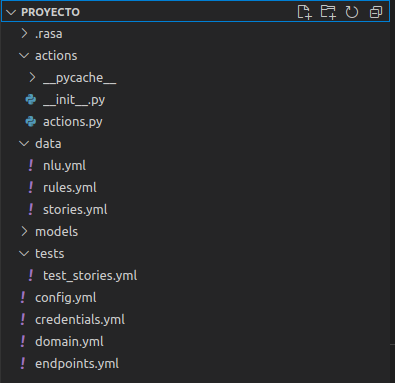
\includegraphics[width=\textwidth]{imagenes/cap3/4_Estructura del Proyecto.png}
	\caption{Estrucutra de los archivos}
	\label{fig:Estructura}
	\cite{Rasa}
\end{figure}
\subsection{Archivo nlu}
En él se encuentran datos estructurados que sirven para entrenar el modelo y luego extraer la
información de los mensajes del usuario. Estos datos son  las intenciones y entidades, también se
pueden agregar expresiones regulares y algunas tablas de búsqueda. \cite{NLU_Documentation}

\subsection{Archivo Rules}
En este archivo se definen las reglas, que no son mas que  tipo de datos de entrenamiento
encargados de describir partes de una conversación que siempre sigue el mismo
camino.\cite{Rules_Documentation}

\subsection{Archivo Stories}
Las historias son un tipo de datos de entrenamiento, se utiliza para entrenar modelos que puedan
generalizar las rutas de conversación. Las entradas del usuario son expresadas mediante intents, y
entitites si es necesario,  mientras que las respuestas del asistente son expresadas mediante
actions.\\
Los patrones que siguen las conversaciones podemos extraer de datos ya existentes o con la
herramienta de rasa 'interactive learning'.\cite{Stories_Documentation}

\subsection{Archivo config}
En el archivo config se definen el lenguaje y los componentes del pipeline, que forman parte de
Rasa NLU y las políticas a ser utilizadas, correspondiente a Rasa NLU.\\
El pipeline es el encargado de definir la dirección de flujo de datos entre los diferentes
componentes, Rasa nos permite configurar cada uno de ellos según nuestras necesidades, de tal forma
que podamos realizar las predicciones de las intenciones y la extracción de las entidades. Las
políticas forman parte de la gestión de diálogos, encargada de seleccionar la siguiente acción a
ser ejecutada.\cite{Configuration_Documentation}\\
La configuración del pipeline y las políticas son de suma importancia, por lo que se detallaran sus
componentes en la sección \ref{ch:Componentes}.

\subsection{Archivo credentials}
Aquí se definen los credenciales para las plataformas de voz y chat que el bot utiliza. Rasa cuenta
con algunos conectores preestablecidos para los canales mas conocidos como Facebook Messenger,
Telegram, Google Hangouts Chat o una pagina web propia.\cite{Credentials_Documentation}

\subsection{Archivo domain}
El archivo domain es un archivo de configuración donde se especifican las intenciones, entidades,
slots, respuestas, formularios y acciones que el bot debe saber.\cite{Domain_Documentation}

\subsection{Archivo endpoints}
Los endpoints son los enlaces a los servicios externos o internos que puede tener Rasa. En el se
definen los servidores que corren o en los que están alojadas las acciones personalizadas, al igual
que los modelos con los que se cuenta. También es aquí donde se especifican los tracker store,
utilizados para guardar las conversaciones, y los event broker, encargados de conectar el bot con
otros servicios que procesan los datos que llegan de las conversaciones.

\section{Componentes}\label{ch:Componentes}
% de https://rasa.com/blog/intents-entities-understanding-the-rasa-nlu-pipeline/
En esta sección estaremos describiendo el funcionamiento de los componentes utilizados en la
arquitectura de Rasa,
estos componentes son modulares y genéricos para lo que son sistemas de NLU modernos, pueden ser
propios del
entorno o proveídos por otras librerías de terceros para extender funcionalidades.

\begin{figure}[h]
	\centering
	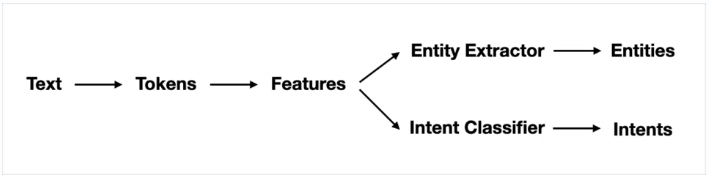
\includegraphics[width=\textwidth]{imagenes/cap3/rasa_components.png}
	\caption{Componentes de un esquema NLU}
	\label{fig:Componentes-MLU}
	\cite{Rasa}
\end{figure}

\subsection{Tokenizadores}
Antes de poder ser procesada una porción de texto debe ser dividida en porciones mas pequeñas, para
esto se suele utilizar
un tokenizador (o tokenizer).	Este divide el texto en componentes de un vector.\\ Algunos
tokenizadores también
agregan información extra a los tokens que pueden ser usados para generar lemas, o sea extraer la
palabra que da el significado base a las palabras que pueden ser utilizados por el contador de
vectores.\\
Para el Inglés y el Español usualmente se usa WhiteSpaceTokenizer que separa en tokens cuando se
detectan espacios, para los idiomas que no precisen de espacios en blanco para separar las palabras
como el Coreano, Japones o Chino, se utilizan MitieTokenizer, en el caso del último tambien es muy
frecuente el uso de JiebaTokenizer.\cite{warmerdam_2022}

\begin{figure}[h]
	\centering
	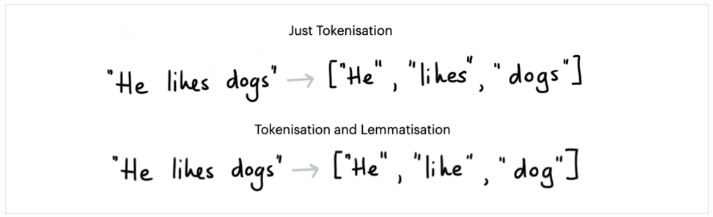
\includegraphics[width=\textwidth]{imagenes/cap3/tokenization.png}
	\caption{Tokenización}
	\label{fig:tokenization-MLU}
	\cite{Rasa}
\end{figure}

\subsection{Caracterizadores}
Los caracterizadores generan pesos numéricos para ser consumidos por los modelos de ML. Existen
dos tipos principales de
características, las Dispersas(Sparse Features) que usualmente cuentan lo que pueden representar
subpalabras o características
léxicas y las Densas(Dense Features) estos suelen consistir en porciones preentrenadas, para que
estos se desempeñen correctamente se debe seleccionar un Tokenizador apropiado.
\cite{warmerdam_2022}
Todos los caracterizadores son presentados en la tabla \ref{tab:Caracterizadores}

\begin{table}[]
	\resizebox{\textwidth}{!}{%
		\begin{tabular}{|l|l|l|}
			\hline
			\textbf{Caracterizador}    & \textbf{Requisitos}     & \textbf{Tipo}
			\\ \hline
			MitieFeaturizer            & MitieNLP                & Dense featurizer
			\\ \hline
			SpacyFeaturizer            & Dense / Sparse Features & \begin{tabular}[c]{@{}l@{}}Logistic
				                                                       Regression de \\ scikit-learn\end{tabular} \\ \hline
			ConveRTFeaturizer          & Tokenization            & Dense featurizer
			\\ \hline
			LanguageModelFeaturizer    & Tokenization            & Dense featurizer
			\\ \hline
			CountVectorsFeaturizer     & Tokenization            & Sparse featurizer
			\\ \hline
			LexicalSyntactitFeaturizer & Tokenization            & Sparse featurizer
			\\ \hline
			RegexFeaturizer            & Tokenization            & Sparse featurizer
			\\ \hline
		\end{tabular}%
	}
	\caption{ Caracterizadores. Elaboración Propia}
	\label{tab:Caracterizadores}
\end{table}

\begin{figure}[h!]
	\centering
	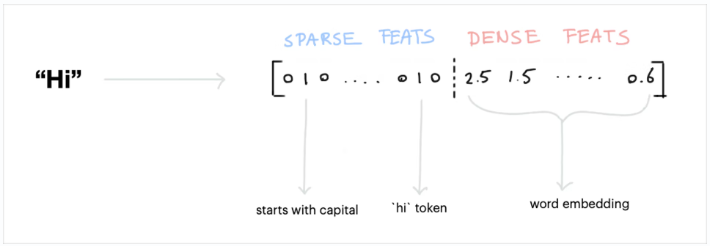
\includegraphics[width=\textwidth]{imagenes/cap3/featurizers.png}
	\caption{Caracterización}
	\label{fig:feazturization-MLU}
	\cite{Rasa}
\end{figure}

\subsection{Clasificadores de Intención(Intent Classiffiers)}

Una vez que se generaron las características para todos los tokens y para toda la oración, podemos
pasarlos a un
modelo clasificador de intenciones. Rasa por defecto usa el modelo DIET que puede encargarse tanto
de
la clasificación de la intención y extracción de entidades. También puede aprender tanto de
características de Tokens como de oraciones. \cite{warmerdam_2022}
% Please add the following required packages to your document preamble:
% \usepackage{graphicx}
\begin{table}[]
	\resizebox{\textwidth}{!}{%
		\begin{tabular}{|l|l|l|}
			\hline
			\textbf{Clasificador}        & \textbf{Requisitos}     & \textbf{Utiliza}
			\\ \hline
			MitieIntentClassifier        & MitieNLP                & Clasificación multiclase con SVM
			\\ \hline
			LogisticRegressionClassifier & Dense / Sparse Features & Logistic Regression de scikit-learn
			\\ \hline
			SklearnIntentClassifier      & Dense Features          & \begin{tabular}[c]{@{}l@{}}SVM lineal
				                                                         optimizado con búsqueda \\ en cuadrícula\end{tabular} \\ \hline
			KeywordIntentClassifier      & Ninguno                 & Comparador de palabras clave
			\\ \hline
			DIETClassifier               & Dense Features          & Transformadores
			\\ \hline
			FallbackClassifier           & Intents                 & \begin{tabular}[c]{@{}l@{}}Requiere de un
				                                                         clasificador de \\ intenciones previo\end{tabular}    \\ \hline
		\end{tabular}%
	}

	\caption{Clasificadores de intenciones. Elaboracion propia}
	\label{IntentClassifier}
\end{table}
\begin{figure}[h]
	\centering
	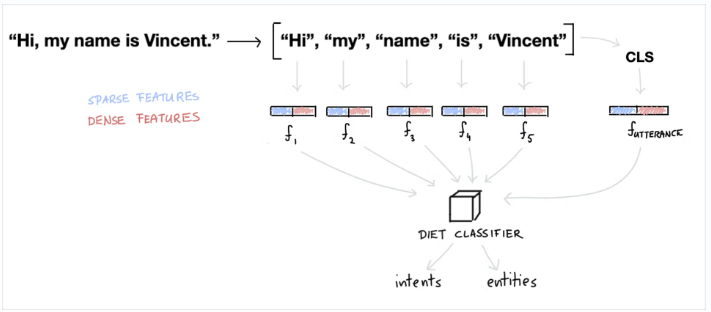
\includegraphics[width=\textwidth]{imagenes/cap3/intent_classiffier.png}
	\caption{Clasificación de intenciones y entidades}
	\label{fig:intentclasification-MLU}
	\cite{Rasa}
\end{figure}

\subsection{Extracción de entidades}

Además de DIET, existen otros clasificadores basados en ML que pueden aprender como detectar
entidades, estos no son recomendados para todos los casos, también puede ser implementado un
extractor basado en Expresiones
Regulares(RegexEntityExtractor) \cite{warmerdam_2022}
% Please add the following required packages to your document preamble:
% \usepackage{graphicx}

\begin{table}[h!]
	\resizebox{\textwidth}{!}{%
		\begin{tabular}{|l|l|l|}
			\hline
			\textbf{Clasificador}   & \textbf{Requisitos} & \textbf{Utiliza}
			\\ \hline
			MitieEntityExtractor    & MitieNLP            & \begin{tabular}[c]{@{}l@{}}Clasificación multiclase
				                                                \\ con SVM\end{tabular} \\ \hline
			SpacyEntityExtractor    & SpacyNLP            & Modelo estadístico BILOU
			\\ \hline
			CRFEntityExtractor      & Tokens              & Campo aleatorio condicional (CRF)
			\\ \hline
			DucklingEntityExtractor & Ninguno             & Expresiones regulares
			\\ \hline
			DIETClassifier          & Dense Features      & Transformadores
			\\ \hline
			RegexEntityExtractor    & Ninguno             & Tablas de búsqueda
			\\ \hline
		\end{tabular}%
	}
	\caption{Extractores de entidades. Elaboración propia}
	\label{EntityExtractor}
\end{table}
\begin{figure}[h]
	\centering
	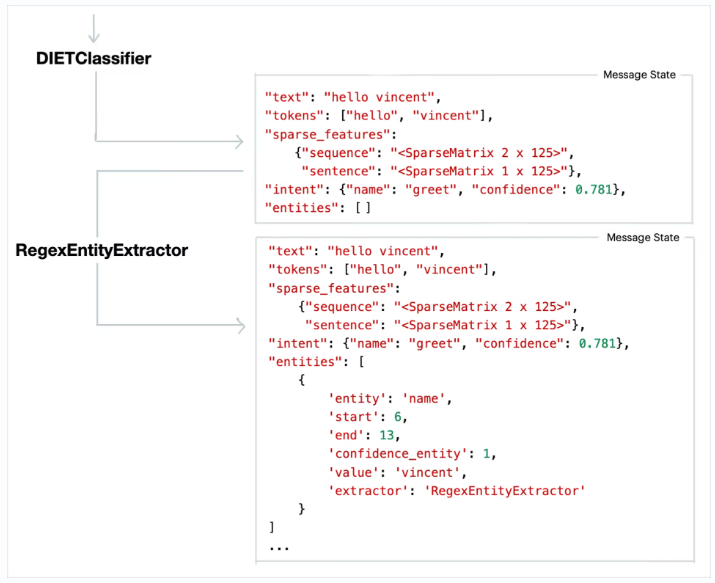
\includegraphics[width=\textwidth]{imagenes/cap3/regex_extractor.png}
	\caption{Extractor Regex}
	\label{fig:regex-extractor}
	\cite{Rasa}
\end{figure}

\subsection{Selectores}
Los selectores se encargan de predecir la respuesta de un conjunto de respuestas posibles para los
retrieval intents, son utilizados posteriormente por el gestor de diálogo para dar la respuesta mas
adecuada.
Utiliza la misma arquitectura y optimización que el DIETClassifier.

\subsection{Predicción de acciones}
\begin{figure}[h!]
	\centering
	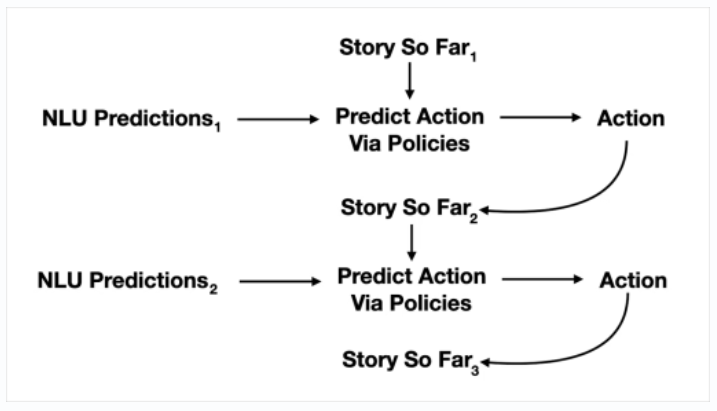
\includegraphics[width=\textwidth]{imagenes/cap3/predicciones.png}
	\caption{Predicción de acciones.}
	\label{fig:regex-extractor}
	\cite{Rasa}
\end{figure}

Con el flujo NLU, se detectan las entidades e intenciones. Pero este flujo no predice la siguiente
acción en la
conversación. Para esto se utiliza el flujo de política. Las políticas aseguran el uso de
predicciones de NLU así como
también el estado presente de la conversaciones para decidir que acción tomar, pueden ser basado en
reglas o en aprendizaje automático.\\
\textbf{Políticas basadas en Aprendizaje Automático:}
\begin{itemize}
	\item \textbf{TED Policy:}
	      Es un conjunto de algoritmos desarrollados por RASA para la predicción de diálogo y
	      reconocimiento de entidades. Su arquitectura se basa en transformadores que convierten el diálogo
	      actual en un vector de diálogos, para compararlos con otros vectores en busca del mas cercano, a
	      partir de las acciones existentes.\cite{ConversationalAIwithRasa}
	\item \textbf{UnexpecTED Intent Policy:} Es una política auxiliar, tiene la misma arquitectura
	      que TEDPolicy pero éste aprende cuales son las intenciones mas probables a ser expresadas según el
	      contexto de la conversación. Siempre debe usarse en conjunto con al menos una otra
	      política.\cite{UnexpecTED}
	\item \textbf{Memoization Policy: }Esta política utiliza las historias y acciones de los datos
	      de entrenamiento y las guarda en un diccionario, si la conversación actual no coincide con ningun
	      ejemplo, predice un 0.0.\cite{MemoizationPolicy}
	\item \textbf{Augmented Memoization Policy: } Tiene las mismas funcionalidades de Memoization
	      Policy, pero además cuenta con un mecanismo que permite olvidar de forma aleatoria algunas partes
	      de la conversación, luego predice las acciones ya con la historia
	      reducida.\cite{AugmentedMemoizationPolicy}
\end{itemize}
\textbf{Políticas basadas en Reglas:}
\begin{itemize}
	\item \textbf{Rule Policy:} Realiza las predicciones basandose en reglas que se tienen en los
	      datos de entramiento.
\end{itemize}
Con cada interacción, las políticas definidas indican con un nivel de confianza cuál será la
siguiente acción a ser tomada, aquella que tiene obtiene el mayor resultado sera la que decida la
siguiente acción, en caso de que se prediga con la misma confianza, se tiene en cuenta la siguiente
asignación de importancia.
\begin{itemize}
	\item 6 - RulePolicy
	\item 3 - MemoizationPolicy o AugmentedMemoizationPolicy
	\item 2 -  UnexpecTEDIntentPolicy
	\item 1 - TEDPolicy
\end{itemize}

\section{Patrones de Conversación}
\subsection{Chitchat y FAQs}
Las preguntas frecuentes y los chitchats (conversaciones sobre temas no importantes) son casos
donde el asistente siempre tiene que responder de la misma forma, sin importar el contexto de la
conversación. El problema se encuentra en que si creamos intenciones y acciones para cada pregunta
que se realiza, las historias y reglas serán muy extensas, es por eso que estas preguntas
frecuentes las agrupamos en una 'retrieval intent' y se selecciona la respuesta correcta mediante
el componente 'Response Selector'.\\
Para poder utilizarlo se debe configurar apropiadamente el archivo config.yml. Este componente
utiliza la política basada en reglas 'RulePolicy', también caracterizadores y clasificadores de
intenciones por lo que debe ubicarse en el pipeline después de estos.
\subsection{Fallbacks}
Para los casos donde el usuario pregunta algo que está fuera del alcance del bot, establecemos una
intención llamada 'out of scope' a la que asociamos a una respuesta genérica y creamos una regla en
el archivo rules.yml.\\ Existen casos donde la confianza en la clasificación es muy baja, esto
implica que no se pueda predecir con buena confianza si se trata de una intención 'out of scope',
para ello Rasa tiene una opción llamada 'Fallback' que permite pedir al usuario que reformule su
pregunta para tratar nuevamente de predecir correctamente a que intención se refiere. \\
Para su utilización se debe agregar el 'FallbackClassifier' en el pipeline, crear respuestas por
defecto y actualizar las reglas.
\section{Pruebas}
Rasa cuenta con varias funciones para probar los diálogos, historias, el gestor de diálogos y el
procesamiento de mensajes.
\subsection{Validación de datos}
El comando 'rasa data validate' se encarga de verificar que no haya errores e inconsistencias en
los datos y configuraciones. Es recomendable ejecutar este comando antes de entrenar el modelo, ya
que si se encuentra algún problema, el entrenamiento también podría fallar.
\subsection{Evaluación del desempeño de la NLU}
Una practica usual al ejecutar aprendizaje automático es dividir aleatoriamente el conjunto de
datos en uno de entrenamiento y otro de pruebas. El bot utiliza el primer conjunto para aprender
las características necesarias para realizar las predicciones adecuadas, y el segundo conjunto para
evaluar el modelo mediante datos que aún no hayan sido vistos antes.\\
Rasa nos permite dividir los datos mediante el comando 'rasa data split nlu' que por defecto separa
los datos de entrenamiento/prueba en un 80/20, luego, para probar que tan bien entrenado se
encuentra el modelo utilizamos 'rasa test nlu' especificando cuales son los datos de entrenamiento
y prueba de la siguiente forma:\\
--nlu train\_test\_split/test\_data.yml

Otro método muy completo para evaluar el modelo es mediante validación cruzada o cross validation.
Este divide los datos en múltiples subconjuntos llamados 'folds' donde se van alternando los datos
de entrenamiento y pruebas

\section{Despliegue del sistema}
Según la documentación de Rasa, el mejor momento para desplegar una versión de prueba es tan rápido
cuando
se tenga un bot que cumpla los requisitos mínimos de los requisitos de diseño. De esta manera se
puede
tener pruebas de usuarios reales lo mas rápido posible y poder agregar estos casos.

\subsection{Arquitectura}

\begin{figure}[h]
	\centering
	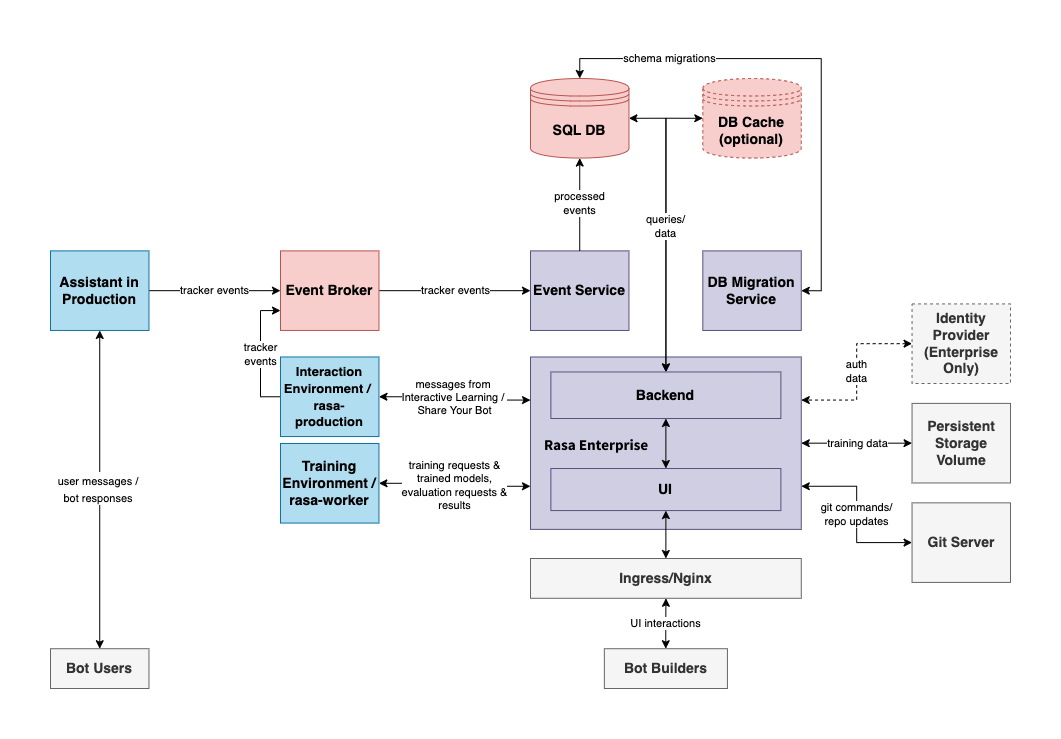
\includegraphics[width=\textwidth]{imagenes/cap3/architecture_deploy.png}
	\caption{Arquitectura}
	\label{fig:deploy-architecture}
	\cite{Rasa}
\end{figure}

\subsubsection{Servicios}
El diagrama muestra tres categorías de servicios: Los morados son componentes de principales de
Rasa
Enterprise, los azules son los servicios principales de Rasa Open Source y los anaranjados son
servicios
de terceros.

Tanto los componentes de Rasa Open Source e Enterprise tienen bases de datos independientes. Los
eventos
datos de conversaciones fluyen desde los servicios de Rasa Open Source a Rasa Enterprise a través
del event broker.

\subsubsection{Servicios de Rasa Enterprise}

Los servicios de Rasa Enterprise, no son todos de libre uso, algunas partes se utilizan bajo un
modelo de
licencias. Pero estos si bien no son indispensables (pueden ser reemplazados por servicios libres
de terceros) hacen que el despliegue de el producto sea mucho mas sencillo y así como también su
desarrollo. Dicho esto pasamos a explicar los existentes en el diagrama, se tratan de los 3 mínimos
servicios para
ejecutar Rasa Enterprise estos deben ser todos de la misma versión para asegurar compatibilidad.

\begin{itemize}
	\item \textbf{Servicio de eventos(Event Service):} Consume datos del corredor de eventos(event

	      broker) y los archiva en la base de datos.
	\item \textbf{Servicio de migración de la Base de datos(DB migration service):}  Asegura que
	      los esquemas de la base de datos
	      esten actualizados con respecto a la versión actual de Rasa Enterprise.
	\item \textbf{Rasa-X:} Ejecuta las tareas del back-end y front-end. Archiva y recupera datos de

	      conversaciones, entrenamiento y meta-datos, como rótulos de conversaciones y banderas de
	      mensajes
	      en la base de datos de Rasa Enterprise. El front-end usa las entradas del back-end para brindar
	      una
	      interfaz amigable para el usuario.
\end{itemize}

\subsubsection{Servicios de Rasa Open Source}

Los servicios de Rasa Open Source se ejecutan de manera totalmente independiente de Rasa
Enterprise,
por otro lado Rasa Enterprise si depende de Rasa Open Source para manejar los datos de las
conversaciones,
entrenamiento y ejecución de modelos. En orden para que Rasa Enterprise pueda mostrar
conversaciones
tomadas por Rasa Open Source este publica los eventos de una conversación a el mismo event broker
al cual Rasa Enterprise esta consumiendo.

\subsubsection{Partes}

\begin{itemize}
	\item \textbf{rasa-production:} Es el servicio que ejecuta el modelo entrenado, usado para
	      parsear mensajes en intents y predecir acciones en conversaciones con el usuario, en un canal
	      o
	      en UI de Rasa Enterprise.
	\item \textbf{rasa-worker:} Es utilizado para servicios de segundo planos, como para entrenar
	      un
	      nuevo modelo.
	\item \textbf{app:} Es el servidor de acciones personalizadas, ejecutan acciones especificas
	      de la aplicación.
\end{itemize}
